\documentclass[11pt]{article}

\usepackage[a4paper,margin=1in,headheight=14pt]{geometry}
\usepackage[T1]{fontenc}
\usepackage{lmodern}
\usepackage{microtype}
\usepackage{amsmath}
\usepackage{amssymb}
\usepackage{amsthm}
\usepackage{booktabs}
\usepackage{array}
\usepackage{enumitem}
\usepackage{caption}
\usepackage{xcolor}
\usepackage{listings}
\usepackage{tikz}
\usepackage[hidelinks,breaklinks]{hyperref}
\usepackage[capitalise,noabbrev]{cleveref}
\usepackage{url}

\usetikzlibrary{positioning,fit,backgrounds,calc,arrows.meta}

\definecolor{kw}{HTML}{0F3D91}
\definecolor{cm}{HTML}{6E7780}
\definecolor{st}{HTML}{147145}

\lstdefinelanguage{json}{
  basicstyle=\ttfamily\footnotesize,
  showstringspaces=false,
  literate=
    *{\{}{{{\color{kw}\{}}}{1}
     {\}}{{{\color{kw}\}}}}{1}
     {[}{{{\color{kw}[}}}{1}
     {]}{{{\color{kw}]}}}{1}
     {:}{{{\color{kw}:}}}{1}
     {,}{{{\color{kw},}}}{1},
  stringstyle=\color{st},
  morestring=[b]"
}

\lstdefinelanguage{rs}{
  basicstyle=\ttfamily\footnotesize,
  keywords={struct,enum,pub,let,fn,impl,trait,use,mod,Option,Result,Vec,String,Some,None,true,false,if,else,match,return,bool,u8,u32,u64,i64,usize,Box,Arc},
  keywordstyle=\color{kw}\bfseries,
  commentstyle=\color{cm}\itshape,
  stringstyle=\color{st},
  showstringspaces=false,
  morecomment=[l]{//},
  morestring=[b]"
}

\lstset{
  basicstyle=\ttfamily\footnotesize,
  columns=fullflexible,
  keepspaces=true,
  xleftmargin=1em,
  frame=none,
  breaklines=true,
  breakatwhitespace=true,
  showstringspaces=false
}

\newtheoremstyle{plainsmall}{0.6\baselineskip}{0.4\baselineskip}{\itshape}{}{\bfseries}{.}{ }{}
\theoremstyle{plainsmall}
\newtheorem{invariant}{Invariant}
\newtheorem{property}{Property}

\title{\bfseries Covenant: A Capability-Based Operating Layer\\for Autonomous Software Engineering Agents}

\author{Achille Wasque\\[2pt]
\small The Covenant Project\\
\small\url{https://opencovenant.org} \quad\textbar\quad \small\url{https://github.com/open-covenant/covenant}}

\date{}

\begin{document}
\maketitle

\begin{abstract}
\noindent Long-running autonomous software agents need infrastructure that their substrate does not provide: scoped authority that can be granted, expired, and revoked; durable project memory that tolerates drift; isolated execution that does not silently degrade; and provenance that binds tasks, code, and validation evidence into one inspectable record. Existing agent frameworks build these properties inside the application, where they are ad-hoc and unauditable; conventional developer environments assume a human operator at every step. We describe \textsc{Covenant}, an open operating layer that exposes eight primitives---intent, runtime, memory, identity, permissions, comms, compositor, settlement---behind a local Rust daemon, with append-only audit and hash-chain integrity underneath. Three load-bearing properties distinguish the design from prevailing agent stacks. First, capability scopes are versioned, signed end-to-end, validated at grant, and \emph{re-checked at dispatch} against per-action predicates. Second, sandbox-required manifests \emph{fail closed} when the active runtime cannot satisfy the declared isolation grade. Third, provenance envelopes bind a task identifier, a Git commit, changed-file evidence, transition events, and validation records into a single object suitable for transparency-log publication. We state the threat model, formalize four invariants on which the system's authority claims rest, and report on the implementation (19 Rust crates, $\sim$62\,000 lines of Rust, 848 tests of which 107 exercise live boundaries against the daemon, CLI, HTTP gateway, MCP adapter, A2A queue, runtime, and selected back-ends). We are explicit about deliberate gaps---production sandboxing for hostile code, multi-peer operation across untrusted hosts, and on-chain settlement---and discuss what is required to close them. Covenant is released under Apache-2.0.
\end{abstract}

\section{Introduction}
\label{sec:intro}

Software agents built on large language models are moving from interactive coding assistance to long-running engineering work: maintaining services, repairing regressions, executing multi-file refactors, and acting on production state through real tools. An agent that runs for an hour is a chat session. An agent that runs for a week is a process with state, authority, and consequences. The infrastructure problem changes accordingly.

Two unmodified substrates currently absorb that load. The first is the developer environment---a shell, a filesystem, a process tree---which assumes a human operator is present at every step to type, confirm, and intervene. Its mechanisms for authority, recovery, and accountability are informal: a human remembers what they ran, why, and where the artifacts went. The second is the agent framework: a library or service that orchestrates prompts, tools, and memory. These frameworks vary in quality, but typically expose memory as an opaque key-value store, authority as a binary toggle, and accountability as application-level logging. Neither substrate gives operators a usable model of what an autonomous agent did, with what authority, and how to verify it later.

Two adjacent communities have already developed strong assumptions about these properties. Operating systems research has decades of work on capability-based authority, audit, and isolated execution~\cite{dennis1966,miller2006,sel4}. Blockchain systems assume verifiable state transitions, explicit authority through cryptographic keys, and attribution down to the level of a single signed message~\cite{nakamoto2008,yakovenko2018}. \textsc{Covenant} is an open operating layer that brings those assumptions into agent infrastructure. It exposes a small set of primitives---intent, runtime, memory, identity, permissions, comms, compositor, settlement---and a cross-cutting audit layer underneath, all mediated by a local Rust daemon called \texttt{covenantd}.

\paragraph{Contributions.} This paper makes the following contributions.

\begin{itemize}[leftmargin=*,itemsep=2pt]
  \item A \textbf{threat model} for long-running autonomous engineering agents that names adversaries (malicious local agent, compromised tool, compromised peer, hostile host kernel), trust boundaries, and explicit security goals (\Cref{sec:threat}).
  \item A \textbf{system architecture} organized around eight primitives plus a cross-cutting audit layer, mediated by a local Rust daemon (\Cref{sec:arch}).
  \item A \textbf{capability model} with versioned scope envelopes, signed end-to-end, validated at grant and re-checked at dispatch against per-action predicates. We formalize this as \emph{Invariant~\ref{inv:dispatch}} (\Cref{sec:caps}).
  \item An \textbf{audit integrity construction}: append-only JSONL with a SHA-256 hash-chain sidecar, retention-aware re-anchoring, and audit-root attestations. We formalize tamper evidence as \emph{Invariant~\ref{inv:tamper}} (\Cref{sec:audit}).
  \item A \textbf{tiered memory model} with three drift predicates that detect inconsistency between memory, audit, capability, and receipt stores in linear time, formalized as \emph{Invariant~\ref{inv:drift}} (\Cref{sec:mem}).
  \item A \textbf{runtime model} with manifest-declared sandbox grades, a trusted-local subprocess back-end, and an opt-in Linux gVisor back-end, with \emph{Invariant~\ref{inv:failclosed}} on fail-closed dispatch (\Cref{sec:runtime}).
  \item A \textbf{provenance envelope} format that binds an autonomy task, a Git commit, changed-file evidence (paths and blob hashes), transition events, and validation records into one inspectable object, and a companion audit-root attestation that links an integrity report to commit or release subjects (\Cref{sec:prov}).
  \item An \textbf{open implementation}: 19 crates, $\sim$62\,000 lines of Rust, 848 tests of which 107 exercise live boundaries; a Next.js operator console; an Anchor settlement program scaffold (\Cref{sec:impl}).
\end{itemize}

\paragraph{Scope.} \textsc{Covenant} is an operating layer, not an agent framework: it does not prescribe a prompting style, a planning algorithm, or a particular tool ontology. It is not an operating system: it runs as an unprivileged daemon on stock Linux or macOS and does not own scheduling, memory protection, or filesystem semantics. It sits between those layers, owning the state, authority, and accountability concerns that recur across agent applications, so individual frameworks can stop reinventing them.

\paragraph{Honest limits.} The local control plane is real and live-tested. Production sandboxing for hostile code, multi-peer operation across untrusted hosts, and on-chain settlement are not. We treat that line as load-bearing: an operating layer that conflates roadmap with implementation is one whose authority claims cannot be trusted. \Cref{sec:limits} discusses what remains.

\section{Threat Model and Design Goals}
\label{sec:threat}

\subsection{Adversaries}
\label{ssec:adversaries}

We consider four adversary classes.

\paragraph{A1: Malicious local agent.} An agent installed on the host that may attempt to escalate beyond its declared capabilities. It can issue arbitrary intents over IPC or HTTP, present forged or replayed tokens, attempt to mutate memory or audit state outside its declared scope, and consume resources beyond its declared budget. It cannot subvert the host kernel; it can attempt to subvert the daemon.

\paragraph{A2: Compromised tool or MCP server.} A tool registered with the daemon whose implementation is hostile or compromised. It can return malformed responses, attempt to widen the effect of a tool call beyond what its capability scope allows, or exfiltrate state passed to it. It cannot forge daemon-side audit rows.

\paragraph{A3: Compromised peer.} A remote peer authenticated to the daemon whose identity key may be valid but whose behavior is hostile. It can attempt to inject A2A messages outside its declared scope, replay messages, or attempt cross-peer authority escalation. The peer-auth boundary is in scope; networked multi-peer operation across untrusted hosts is roadmap.

\paragraph{A4: Compromised host kernel.} Out of scope. If the kernel is owned, primitives that rely on file integrity, process isolation, or memory protection fail. We name this explicitly because security claims at the local control plane do not generalize beyond it.

\subsection{Trust Boundaries}
\label{ssec:trust}

\Cref{tab:trust} enumerates the trust boundaries the system claims to enforce and the mechanism that enforces each.

\begin{table}[h]
\centering
\caption{Trust boundaries and enforcement mechanisms.}
\label{tab:trust}
\small
\begin{tabular}{@{}lp{0.36\linewidth}p{0.36\linewidth}@{}}
\toprule
ID & Boundary & Enforcement \\
\midrule
B1 & Host kernel $\leftrightarrow$ agent process & gVisor user-space kernel for opt-in dispatch; trusted-local otherwise (no kernel-level claim). \\
B2 & Agent $\leftrightarrow$ daemon state mutation & Signed capability tokens with dispatch-time scope predicates. \\
B3 & Agent $\leftrightarrow$ tool effect & Tool-call argument allowlist on \texttt{tool.call.<name>}; daemon-side schema validation on results. \\
B4 & Agent $\leftrightarrow$ external credential & Daemon brokers; agent never sees raw credentials. (Implementation is partial; see \Cref{sec:limits}.) \\
B5 & Local audit $\leftrightarrow$ on-disk corruption & SHA-256 hash chain over the retained JSONL log; retention purge re-anchors. \\
B6 & Local audit $\leftrightarrow$ remote verification & Audit-root attestations bound to commits or release subjects; transparency-log publication is open. \\
B7 & Peer $\leftrightarrow$ peer authority & Peer-scoped capability predicates for A2A send, receive-admission, respond, and repair; operator tokens rotatable, mode-0600 on disk. \\
\bottomrule
\end{tabular}
\end{table}

\subsection{Security Goals}
\label{ssec:goals}

\begin{description}[leftmargin=2.5em,itemsep=2pt]
  \item[\textbf{G1 Authority Containment.}] An agent's effect is bounded by its declared and currently-valid capabilities; long-lived tokens do not become ambient authority.
  \item[\textbf{G2 Tamper-Evident Audit.}] Any modification of the retained audit log on disk is detectable by local verification, and audit roots are bindable to commits and release subjects for off-host verification.
  \item[\textbf{G3 Drift Detection.}] Inconsistencies between memory, audit, capability, and receipt stores are detectable in time linear in the size of the stores.
  \item[\textbf{G4 Fail-Closed Isolation.}] A manifest that declares a sandbox grade is honored at dispatch or refused; the system does not silently downgrade isolation.
  \item[\textbf{G5 Attributable Action.}] Every privileged action carries a signed audit row sufficient to attribute it to a subject, an action, a scope, and a result.
\end{description}

\subsection{Non-goals}
\label{ssec:nongoals}

We do not claim full autonomous software engineering without human authority, production sandbox-grade isolation against arbitrary hostile agent code (the trusted-local back-end is explicitly not a security boundary against such code), production multi-peer operation across untrusted hosts, production on-chain settlement, or a benchmarked self-improvement loop. These appear as roadmap where relevant.

\section{System Overview}
\label{sec:arch}

The center of the system is \texttt{covenantd}, a Rust daemon that owns local state and mediates privileged operations. Clients reach the daemon through IPC frames over a Unix socket, a local HTTP gateway, or the \texttt{covenant} CLI. Agents reach the daemon through the same surfaces or through manifest-declared protocols. Eight primitives are exposed through the daemon; audit underlies them.

\begin{figure}[h]
\centering
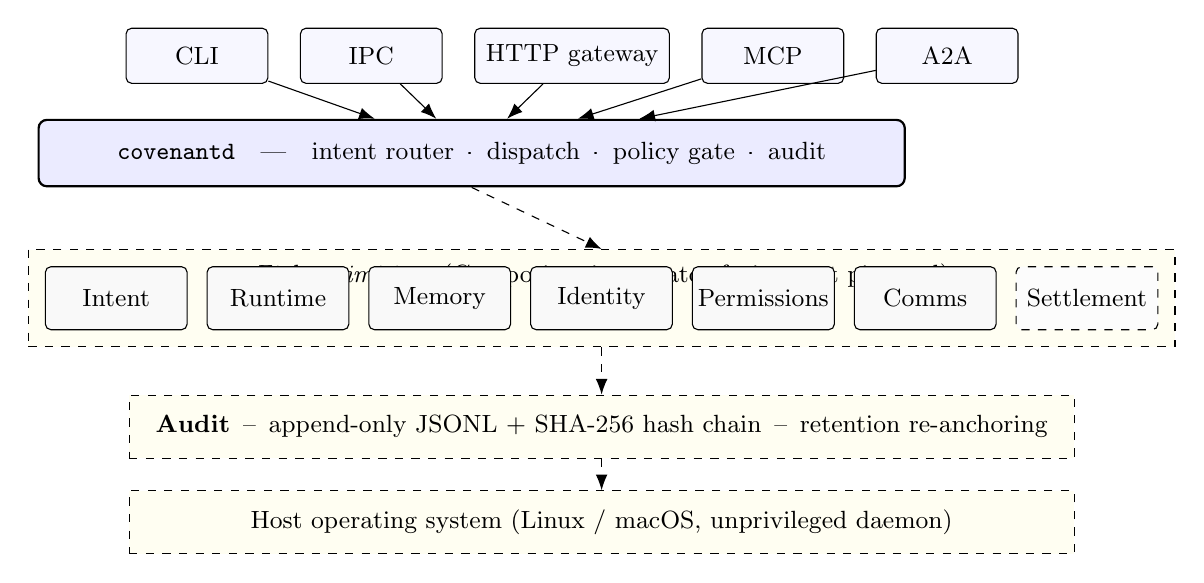
\begin{tikzpicture}[
  font=\small,
  every node/.style={align=center},
  block/.style={rectangle,draw,rounded corners=2pt,inner sep=4pt,minimum height=7mm,minimum width=18mm,fill=blue!3},
  daemon/.style={rectangle,draw,thick,rounded corners=3pt,inner sep=8pt,fill=blue!8},
  prim/.style={rectangle,draw,rounded corners=2pt,minimum width=18mm,minimum height=8mm,inner sep=2pt,fill=gray!5},
  host/.style={rectangle,draw,dashed,inner sep=5pt,fill=yellow!5},
  link/.style={-{Latex[length=2mm]}},
  >=Latex
]
\node[block] (cli) {CLI};
\node[block,right=4mm of cli] (ipc) {IPC};
\node[block,right=4mm of ipc] (http) {HTTP gateway};
\node[block,right=4mm of http] (mcp) {MCP};
\node[block,right=4mm of mcp] (a2a) {A2A};

\node[daemon,below=8mm of $(ipc)!0.5!(http)$,minimum width=110mm] (d)
  {\textbf{\texttt{covenantd}}\quad\textemdash\quad intent router \,\textperiodcentered\, dispatch \,\textperiodcentered\, policy gate \,\textperiodcentered\, audit};

\node[prim,below=10mm of d.south west,xshift=10mm] (intent) {Intent};
\node[prim,right=2.4mm of intent] (rt) {Runtime};
\node[prim,right=2.4mm of rt] (mem) {Memory};
\node[prim,right=2.4mm of mem] (id) {Identity};
\node[prim,right=2.4mm of id] (perm) {Permissions};
\node[prim,right=2.4mm of perm] (comms) {Comms};
\node[prim,right=2.4mm of comms,fill=gray!2,dashed] (set) {Settlement};

\begin{scope}[on background layer]
\node[host,fit=(intent)(set),inner sep=6pt,label={[anchor=north,xshift=0pt,yshift=-2pt]north:\textit{Eight primitives} (Compositor is operator-facing; not pictured)}] (primbox) {};
\end{scope}

\node[host,below=6mm of primbox,minimum width=120mm,minimum height=8mm] (audit) {\textbf{Audit} \,\textendash\, append-only JSONL + SHA-256 hash chain \,\textendash\, retention re-anchoring};

\node[host,below=4mm of audit,minimum width=120mm,minimum height=8mm] (kernel) {Host operating system (Linux / macOS, unprivileged daemon)};

\draw[link] (cli) -- (d);
\draw[link] (ipc) -- (d);
\draw[link] (http) -- (d);
\draw[link] (mcp) -- (d);
\draw[link] (a2a) -- (d);
\draw[link,dashed] (d.south) -- (primbox.north);
\draw[link,dashed] (primbox.south) -- (audit.north);
\draw[link,dashed] (audit.south) -- (kernel.north);
\end{tikzpicture}
\caption{\textsc{Covenant} architecture. The daemon mediates client surfaces (CLI, IPC, HTTP, MCP, A2A) and dispatches through eight primitives over a cross-cutting audit layer. The compositor surface (operator console) is not shown. The settlement primitive is scaffolding (\Cref{sec:settle}).}
\label{fig:arch}
\end{figure}

\Cref{tab:primitives} summarizes the eight canonical primitives. The ordering is canonical: documentation that ships with six or seven is wrong and should be reconciled with this taxonomy.

\begin{table}[h]
\centering
\caption{Canonical primitives. Audit (not listed) underlies Identity, Permissions, and Settlement.}
\label{tab:primitives}
\small
\begin{tabular}{@{}llp{0.58\linewidth}@{}}
\toprule
\# & Primitive & Role \\
\midrule
1 & Intent       & Normalized request shapes for CLI, IPC, HTTP, routing, and daemon dispatch. \\
2 & Runtime      & Agent execution with timeout enforcement, manifest contracts, trusted-local subprocesses, opt-in Linux gVisor back-end. \\
3 & Memory       & SQLite-backed working, episodic, and long-term records with embedding hooks, ignore rules, drift reports, repair, and bounded compaction. \\
4 & Identity     & Local ed25519 identity, peer registry, operator tokens, token rotation, peer revocation. \\
5 & Permissions  & Signed capabilities with versioned scope envelopes, grant-time validation, dispatch-time predicates, expiry, and revocation tombstones. \\
6 & Comms        & IPC frames, local HTTP gateway, MCP adapter, A2A mailbox primitives. \\
7 & Compositor   & Operator console (Next.js) and public documentation surface. \\
8 & Settlement   & Local resource receipts and protocol scaffolding for agent coordination economics. \\
\bottomrule
\end{tabular}
\end{table}

\paragraph{Dispatch flow.} A representative privileged action follows the path:
\begin{enumerate}[leftmargin=*,itemsep=0pt]
  \item A caller submits an intent (CLI, IPC frame, or HTTP request).
  \item The router normalizes it into the typed shape and resolves it to an agent and an action $a$ in a known namespace.
  \item The daemon validates the presented capability $\kappa$: signature, subject match, expiry, revocation tombstone check, and the scope predicate $P_a$ against runtime arguments.
  \item If authorized, the daemon dispatches the action through the appropriate runtime back-end, MCP adapter, A2A queue, or internal handler.
  \item Receipts and audit events are written; the result is returned.
\end{enumerate}

Authority is not implicit in being able to reach the daemon; it is checked at dispatch.

\section{Capability Model}
\label{sec:caps}

\textsc{Covenant} uses a capability model in the tradition of Dennis and Van Horn~\cite{dennis1966} and the object-capability work of Miller~\cite{miller2006}, instantiated as signed tokens with versioned scope envelopes. The structural choice closest to ours is macaroons~\cite{macaroons}, with two adaptations: scope is a typed JSON envelope rather than a sequence of caveats, and predicates are resolved by the issuing daemon rather than by third-party verifiers.

\subsection{Token Shape}

A capability $\kappa$ binds five fields into one signed object: a subject (the agent permitted to use it), an action $a$ (a dotted string in a reserved namespace), an optional JSON scope $s$, an issuer, and an optional expiry. The signature uses Ed25519~\cite{ed25519} and covers the canonical encoding of $(subject, a, s, issuer, expiry)$, so scope fields are tamper-evident.

\begin{lstlisting}[language=rs]
pub struct Capability {
    pub subject:    AgentId,
    pub action:     String,           // e.g. "memory.read.episodic"
    pub scope:      serde_json::Value,
    pub granted_by: AgentId,
    pub expires_at: Option<u64>,
}
\end{lstlisting}

Reserved namespaces include \texttt{intent.*}, \texttt{memory.*}, \texttt{identity.*}, \texttt{tool.*}, \texttt{agent.*}, \texttt{audit.*}, \texttt{chain.*}, and \texttt{peer.*}.

\subsection{Scope Envelope}

Every non-empty scope for a known action namespace must be a JSON object with a version field:

\begin{lstlisting}[language=json]
{ "version": 1 }
\end{lstlisting}

The empty object is valid and means \emph{unscoped within the named action}. Grant requests for known namespaces reject non-object scopes, missing versions, unsupported versions, and malformed known fields. Unknown future fields are preserved as signed metadata until dispatch-time enforcement defines them. This shape keeps capabilities forward-compatible without giving up signature coverage.

For tool invocation, scope can carry an exact argument allowlist:

\begin{lstlisting}[language=json]
{
  "version": 1,
  "tool": "echo",
  "arguments": { "allow": { "text": "constant or policy-owned value" } }
}
\end{lstlisting}

When present on \texttt{tool.call.<name>}, the daemon rejects calls whose full argument object does not exactly match the allowlist. Live HTTP coverage pins this contract: a scoped grant rejects a mismatched argument object before dispatch and permits only the exact allowed object.

For memory operations, scope predicates carry the tier, optional record identifier, optional \texttt{before\_ms} cutoff, and an \texttt{apply} flag distinguishing dry-run from applied repair:

\begin{lstlisting}[language=json]
{
  "version": 1,
  "tiers": ["episodic"],
  "record_id": null,
  "before_ms": null,
  "apply": false
}
\end{lstlisting}

\subsection{Dispatch-Time Predicates}

Grant-time validation alone is insufficient. A token signed for \texttt{memory.read.episodic} with scope \texttt{\{record\_id: r0\}} must not be honored at the moment of dispatch if the request asks for a different record. The daemon therefore re-checks per-namespace predicates at dispatch:

\begin{itemize}[leftmargin=*,itemsep=0pt]
  \item \texttt{memory.read.<tier>}: tier match and record-identifier match;
  \item \texttt{tool.call.<name>}: exact argument-object match against \texttt{arguments.allow};
  \item \texttt{audit.purge}: \texttt{before\_ms} cutoff lower-bound;
  \item \texttt{chain.receipts.read} and \texttt{chain.batches}: receipt-scope predicates (resource, cluster, batch, payer match);
  \item \texttt{a2a.*}: peer-scope predicates for send, receive-admission, respond, and repair;
  \item \texttt{peer.*}: delegated list/revoke predicates with retention bounds.
\end{itemize}

We can now state the load-bearing property.

\begin{invariant}[Dispatch-time authority check]
\label{inv:dispatch}
For every privileged action $a$ in a known namespace dispatched by \texttt{covenantd}, there exists a capability $\kappa$ such that:
(a)~$\kappa$ is signature-valid under an issuer public key in the daemon's identity registry;
(b)~$\mathrm{subject}(\kappa)$ equals the caller's authenticated identity;
(c)~$\mathrm{expiry}(\kappa)$, if present, exceeds the current wall-clock time;
(d)~no revocation tombstone names $\kappa$ in the retained audit log;
(e)~the scope predicate $P_a(\mathrm{scope}(\kappa), \mathrm{args})$ holds for the runtime arguments of $a$.
A failure of any clause causes dispatch refusal and a \texttt{CapabilityCheck} (or scope-specific) audit row.
\end{invariant}

\subsection{Revocation and Rotation}

Revocation is implemented as tombstones in the same audit stream as grants: a revocation event names the token (or token prefix) and is honored at dispatch via clause~(d). Operator-token rotation is supported with mode-0600 enforcement on disk, signed transitions, and explicit reject paths (\texttt{OperatorTokenRotated}, \texttt{OperatorTokenRotationRejected}). The daemon refuses to read or write operator tokens whose on-disk mode is wider than 0600, and refuses to follow symlinks.

\section{Audit Integrity}
\label{sec:audit}

Daemon audit events are recorded as JSONL: one event per line, append-only, tail-friendly. Each event carries a UUID, a millisecond timestamp, and a typed \texttt{AuditKind} payload. The retained log $L$ is paired with a hash-chain sidecar $C$ for tamper evidence.

\subsection{Chain Construction}

For the default \texttt{events.jsonl}, the sidecar is \texttt{events.chain.jsonl}. Each row is an \texttt{AuditChainEntry}:

\begin{lstlisting}[language=rs]
pub struct AuditChainEntry {
    pub index:              u64,    // zero-based position in the retained log
    pub event_id:           Uuid,   // event UUID from the audit row
    pub timestamp_ms:       i64,    // event timestamp from the audit row
    pub event_hash_hex:     String, // SHA-256 of the retained JSONL event line
    pub previous_hash_hex:  String, // previous chain root, or sixty-four zeroes
    pub chain_hash_hex:     String, // SHA-256(previous_hash_hex + "\n" + event_hash_hex)
}
\end{lstlisting}

The chain is a hash list: $c_i = H(c_{i-1} \,\Vert\, \texttt{"\textbackslash n"} \,\Vert\, H(e_i))$ with $c_{-1} = 0^{64}$. The sidecar is append-only under normal writes. If the sidecar is missing or has a different length from the event log at write time, the daemon rebuilds it over the retained events before appending the new anchor. Retention purge rewrites both files so a valid retained log remains valid after old rows are intentionally removed.

\subsection{Tamper Evidence}

Tamper evidence reduces to standard hash-chain properties under SHA-256's collision resistance.

\begin{property}[Local tamper evidence]
\label{inv:tamper}
Let $L = (e_0, \dots, e_n)$ be the retained log and $C = (c_0, \dots, c_n)$ its sidecar produced by the construction above. Under SHA-256 collision resistance:
(i)~any modification, insertion, or deletion of an event $e_i$ that is not accompanied by a rewrite of every $c_j$ for $j \geq i$ produces a verification failure;
(ii)~any rewrite of $C$ inconsistent with $L$ produces a verification failure;
(iii)~deletion of a tail $e_k, \dots, e_n$ and the corresponding $c_k, \dots, c_n$ is detectable only against external commitment to $c_n$.
\end{property}

Clause~(iii) is the load-bearing limit. Hash chains defend against tampering only up to a known root; defending against silent tail truncation requires an external commitment. Audit-root attestations (\Cref{sec:prov}) provide that commitment by binding $c_n$ to a Git commit or release subject, and---once a transparency log is selected---to a publicly observable position.

\subsection{Audit Event Taxonomy}

The \texttt{AuditKind} enum names the typed payloads of audit events. \Cref{tab:audit-kinds} samples the kinds that are stable in the current implementation. The taxonomy is intentionally split: scope-rejection rows, capability-check rows, and authentication-failure rows are distinct kinds, because operator triage of misconfiguration differs from triage of policy rejection.

\begin{table}[h]
\centering
\caption{Representative \texttt{AuditKind} variants. The implementation contains additional kinds for budget exhaustion, chain corruption, peer revocation, memory repair, A2A repair, and operator-token transitions.}
\label{tab:audit-kinds}
\small
\begin{tabular}{@{}lp{0.62\linewidth}@{}}
\toprule
Variant & Meaning \\
\midrule
\texttt{IntentDispatched}              & An intent was routed and dispatched. \\
\texttt{IntentIgnored}                 & An intent matched \texttt{.covenantignore}; no memory or receipt written. \\
\texttt{CapabilityGranted}             & A capability was signed and persisted. \\
\texttt{CapabilityScopeRejected}       & A grant was rejected for scope-envelope violation. \\
\texttt{CapabilityCheck}               & A capability was checked at dispatch (pass or fail). \\
\texttt{AuthenticationFailed}          & A peer or operator failed identity authentication. \\
\texttt{PeerRevoked}                   & A peer registration was revoked. \\
\texttt{BudgetExhausted}               & A budget bound was reached; a pause checkpoint was queued. \\
\texttt{ChainCorruption}               & Audit chain verification detected an inconsistency. \\
\bottomrule
\end{tabular}
\end{table}

\section{Memory Model}
\label{sec:mem}

Long-running engineering agents need durable project context. Without it, every session reconstructs the same understanding from scratch and drifts quickly from the codebase. \textsc{Covenant} exposes three memory tiers and a drift discipline over them.

\subsection{Tiers}

The \texttt{covenant-memory} crate owns three SQLite-backed stores:

\begin{itemize}[leftmargin=*,itemsep=0pt]
  \item \textbf{Working.} Short-lived session context; cleared at session end by default.
  \item \textbf{Episodic.} Records of past tasks, decisions, and reviews, scoped to the project.
  \item \textbf{Long-term.} Stable knowledge about the codebase and operational conventions.
\end{itemize}

Each \texttt{MemoryRecord} carries an embedding, structured metadata, an owner, an optional parent (for derived memories), and a created-at timestamp:

\begin{lstlisting}[language=rs]
pub struct MemoryRecord {
    pub id:         Uuid,
    pub tier:       MemoryTier,        // Working | Episodic | LongTerm
    pub owner:      AgentId,
    pub text:       String,
    pub embedding:  Vec<f32>,
    pub metadata:   serde_json::Value,
    pub created_at: u64,
    pub parent:     Option<Uuid>,
}
\end{lstlisting}

\subsection{Drift, Repair, and Compaction}

The principal hazard of durable memory is drift: records referencing files that no longer exist, identifiers that have been renamed, or claims contradicting current state. A planner that consumes drifted memory cannot distinguish stale references from fresh ones. We treat drift as a first-class object.

\begin{invariant}[Drift detectability]
\label{inv:drift}
Let $M$ be the set of retained memory records, $A$ the retained audit log, $K$ the set of retained capability records, and $R$ the set of retained settlement receipts. The verifier $\mathrm{drift}(M, A, K, R)$ runs in $O(|M| + |A| + |K| + |R|)$ and reports:
(i)~every $m \in M$ whose audit-attributed source is missing from $A$ (\emph{memory $\leftrightarrow$ audit});
(ii)~every $k \in K$ whose grant or revocation event is missing from $A$ (\emph{capability $\leftrightarrow$ audit});
(iii)~every $r \in R$ whose corresponding memory write is missing from $M$ (\emph{memory $\leftrightarrow$ receipts}).
\end{invariant}

The \texttt{covenant verify} command exposes these three predicates. Repair flows are scoped capability actions (\texttt{memory.repair.dry\_run}, \texttt{memory.repair.apply}) so an automated maintenance loop can address drift without escalating to unbounded write authority. Compaction (\texttt{memory.compact.dry\_run}, \texttt{memory.compact.apply}) collapses stale or redundant records under a bounded policy; the policy preserves the provenance of compacted records so an audit reader can recover which records contributed to a compacted summary.

\subsection{Ignore Rules}

A \texttt{.covenantignore} file expresses project-level allow/deny rules for memory auto-ingestion and tool scans. The matcher follows gitignore conventions. Ignored intents skip both memory and receipt writes and emit an \texttt{IntentIgnored} audit row. This is the project-level analogue to \texttt{.gitignore}: a place to say \emph{do not remember this}.

\section{Runtime and Isolation}
\label{sec:runtime}

\textsc{Covenant} separates two questions: which runtime back-end dispatches an agent, and which isolation contract the agent's manifest declares.

\subsection{Manifests}

An agent ships with an \texttt{agent.toml} that declares its runtime (\texttt{python3}, \texttt{node}, \texttt{rust-bin}), entry point, required and optional capabilities, resource bounds, and an optional \texttt{[sandbox]} section:

\begin{lstlisting}[language=rs]
[sandbox]
required = true
backend  = "linux-gvisor"
filesystem = "read-only-package"
network    = "off"
\end{lstlisting}

The \texttt{covenant-manifest} crate refuses to validate manifests that declare \texttt{required = true} without naming a sandbox-grade back-end.

\subsection{Back-ends}

The default back-end is \texttt{trusted-local}: agents run as bounded subprocesses of the daemon, with a wall-clock timeout, stdout and stderr capture, and audit attribution. Trusted-local is useful for first-party automation and local development. \emph{It is not a security boundary against hostile agent code}. It protects daemon-mediated state through capability checks; it does not protect host filesystem reads, inherited environment variables, network access beyond what the host allows, or syscall-level abuse. The threat model (\Cref{ssec:adversaries}) explicitly notes this.

The opt-in back-end is \texttt{linux-gvisor}, which prepares a restrictive OCI bundle and invokes \texttt{runsc}~\cite{gvisor}. The initial runner supports \texttt{filesystem = "read-only-package"} and \texttt{network = "off"} only; broader policies (\texttt{outbound-https-only}, \texttt{full}, \texttt{ephemeral}, \texttt{host}) fail closed pending implementation and validation. The back-end is selected at daemon startup through \texttt{COVENANT\_RUNTIME\_BACKEND}; configuration errors fail startup rather than silently downgrading.

\subsection{Fail-Closed Dispatch}

The load-bearing invariant is fail-closed sandbox semantics. Let $\preceq$ be the partial order on back-ends induced by isolation grade, with $\texttt{trusted-local} \not\preceq \texttt{linux-gvisor}$.

\begin{invariant}[Fail-closed sandbox dispatch]
\label{inv:failclosed}
For every dispatch of an agent whose manifest declares $\mathrm{sandbox.required} = \top$ with back-end $b$, let $b'$ be the active runtime back-end. Dispatch proceeds only if $b \preceq b'$ \emph{and} $b'$ implements the declared $\mathrm{filesystem}$ and $\mathrm{network}$ policies; otherwise dispatch is refused and a \texttt{CapabilityCheck} (or runtime-specific) audit row is emitted. The system does not downgrade isolation to satisfy a manifest's required clause.
\end{invariant}

This matters because the alternative---silent downgrade---is the most common way capability claims in agent infrastructure are quietly broken in practice. A manifest that says \emph{sandbox required} must mean it at dispatch.

\subsection{Budgets and Pause Checkpoints}

The \texttt{covenant-budget} crate maintains a per-agent resource ledger with daemon-backed pause checkpoints. When an agent reaches a declared budget bound, the runtime pauses, persists partial state, settles consumed credits to a local receipt, and queues a resume. Pause checkpoints are validated against three guards: a version match, a non-zero-credits requirement, and a machine-local-path guard that refuses to resume into a checkpoint whose recorded paths disagree with the current host. A failed validation emits a \texttt{BudgetUnseeded} audit row and refuses resume.

\section{Comms: Brokered Surfaces}
\label{sec:comms}

\textsc{Covenant} brokers two external surfaces and one internal one. The shared architectural property is that agents reach external state through brokered interfaces---not ambient host access---so the daemon can apply capability checks and produce attributable audit rows at every boundary.

\paragraph{IPC and local HTTP gateway.}
The daemon exposes IPC frames over a Unix socket under \texttt{\$COVENANT\_HOME} and a local HTTP gateway for browser-and-tool integrations. The gateway is scoped by operator tokens (mode 0600 on disk, refused if wider; symlinks refused) and CORS origins read from the environment at startup. Operator-token presentation gates write surfaces; read surfaces remain capability-checked.

\paragraph{MCP adapter.}
The \texttt{covenant-mcp} crate bridges the Model Context Protocol~\cite{mcp}, a JSON-RPC tool-call protocol now adopted across multiple agent platforms. Tool-call results are validated against declared schemas. Calls are gated at dispatch by the \texttt{tool.call.<name>} predicate against the \texttt{arguments.allow} field of the presented capability.

\paragraph{A2A mailbox.}
The \texttt{covenant-a2a} crate implements a mailbox for agent-to-agent messages~\cite{a2a}, with peer-scoped capability predicates for send, receive-admission, respond, and repair. Queue semantics include idempotent enqueue, lease guards on receive, requeue on force-error, and machine-readable queue-status reads. Each transition is audited; live CLI fixtures pin requeue, force-error repair, and lease behavior.

\section{Provenance Envelopes}
\label{sec:prov}

Provenance is the bridge between local audit and external verification. We define two envelope formats and a verifier.

\subsection{Task Envelopes}

A task envelope binds five fields:

\begin{lstlisting}[language=json]
{
  "task":     "memory-drift-repair",
  "commit":   "20ff55e",
  "evidence": [
    { "path": "agent-os/crates/covenant-memory/src/drift.rs",
      "blob": "9b1e..." }
  ],
  "transitions": [
    { "kind": "IntentDispatched", "event_id": "...", "timestamp_ms": ... },
    { "kind": "CapabilityGranted", "event_id": "...", "timestamp_ms": ... }
  ],
  "validation": { "command": "bash agent-os/scripts/validate.sh --quick",
                  "outcome": "passed" }
}
\end{lstlisting}

The verifier (\texttt{agent-os/scripts/provenance.mjs}) supports three modes: \texttt{write}, \texttt{verify}, and \texttt{verify-all}. \texttt{verify-all} runs as part of the local validation script, so committed envelopes are checked in normal CI. Unsigned envelopes are the default; signed envelopes use detached Ed25519 signatures with a published key id, and the verifier accepts an approved-key set at run time.

\subsection{Audit-Root Attestations}

An audit-root attestation binds the local \texttt{AuditIntegrityReport} (the report produced by \texttt{covenant audit verify}) to either a commit and task or to a release subject. The verifier accepts both shapes:

\begin{lstlisting}
covenant audit verify > audit-report.json

node agent-os/scripts/provenance.mjs audit-root write \
  --report audit-report.json \
  --release v0.1.0-alpha.1 \
  --release-subject release-subject.json \
  --commit HEAD \
  --signing-key ./secure/project-audit-root-key.pem \
  --key-id covenant-root \
  --out docs/provenance/audit-roots/<commit>-audit-root.json \
  --validation "covenant audit verify=passed"
\end{lstlisting}

Audit-root attestations are the artifact that crosses the host boundary. They let a third party verify, against a published key and (when present) a transparency target, that a particular audit log existed at a particular commit. We treat audit roots as the seam between local integrity and public attestation.

\subsection{Transparency Target}

Release-readiness for public provenance is gated on three contracts: artifact subject verification (landed), project key custody (landed), and transparency-log publication (open). Until a published log exists, audit-root attestations are useful for local audit and as a building block for a future verifier, but they do not give a remote party the property they need: an append-only, tamper-evident log they did not have to trust the producer to maintain. The natural targets are Sigstore Rekor~\cite{sigstore} and Trillian-backed logs in the in-toto~\cite{intoto} family.

\section{Settlement: Local Receipts and Protocol Scaffolding}
\label{sec:settle}

Long-running agents consume resources: compute, memory writes, tool calls, A2A messages, registrations. Without an accounting layer, that consumption is invisible; without a settlement layer, it cannot be exchanged across actors. We treat settlement as scaffolding in the current system and are explicit about that line.

\subsection{Receipts}

A \texttt{SettlementReceipt} records a single consumption event:

\begin{lstlisting}[language=rs]
pub struct SettlementReceipt {
    pub id:                Uuid,
    pub payer:             AgentId,
    pub resource:          ResourceKind,    // Compute | Memory | Tool | Message | Registration
    pub credits_consumed:  u64,             // USD-pegged credits destroyed at this event
    pub settled_at:        u64,
    pub memory_record_id:  Option<Uuid>,    // set when resource == Memory
    pub onchain_sig:       Option<String>,  // None until a batched burn lands
}
\end{lstlisting}

Receipts are produced by the daemon and flushed to a local store. They are reachable through capability-scoped \texttt{chain.*} predicates, so automated readers see only the receipts they are authorized to.

\subsection{Protocol Scaffolding}

A Solana~\cite{yakovenko2018} settlement program is scaffolded under \texttt{programs/settlement} with an Anchor build pipeline. The design pairs a fixed-supply token with a USD-pegged credits unit minted by the settlement program at a Pyth oracle rate or USDC 1:1. Credits are destroyed at the moment of resource consumption---the receipt records that destruction event. Provider payouts settle in USDC by default with an optional buyback path. A treasury accrues a fixed portion of credit-mint inflow and runs probabilistic buyback-and-burn.

This is scaffolding. The interface trait ships with a no-op implementation; the first burn surface (memory writes) is local-accounted and queued; on-chain wiring is roadmap. The paper does not claim production on-chain settlement.

\subsection{Why Settlement Is a Primitive}

A reader may ask why an operating layer for agent engineering needs settlement at all. Two answers. \emph{Structurally}: when authority is explicit and accountability is auditable, resource consumption is already legible per receipt; an exchange layer is the natural way to coordinate multi-actor work. Retrofitting it later is worse than scaffolding it now. \emph{Operationally}: a credit-mint and burn record gives the audit layer a quantitative axis (consumed credits per receipt) that is otherwise absent. We are willing to defend the claim that settlement belongs in the canonical eight independently of the specific on-chain mechanism.

\section{Implementation and Measurements}
\label{sec:impl}

\paragraph{Codebase.} The primary implementation is the \texttt{agent-os} Rust workspace: 19 crates totaling $\sim$61\,500 lines of Rust. \Cref{tab:crates} lists the principal crates by line count. The daemon (\texttt{covenantd}) is the largest at $\sim$32\,000 lines and aggregates protocol dispatch, gateway surfaces, integration glue, and validation tests. The remaining crates are focused libraries.

\begin{table}[h]
\centering
\caption{Principal crates in the \texttt{agent-os} Rust workspace, by line count.}
\label{tab:crates}
\small
\begin{tabular}{@{}lr l@{}}
\toprule
Crate & Lines & Role \\
\midrule
\texttt{covenantd}            & 32\,346 & Daemon: router, dispatch, gateway, audit glue, validation \\
\texttt{covenant}             &  6\,237 & CLI \\
\texttt{covenant-tui}         &  4\,611 & TUI scaffolding \\
\texttt{covenant-a2a}         &  2\,613 & A2A mailbox, queue, repair \\
\texttt{covenant-permissions} &  2\,489 & Capabilities: grant, scope, dispatch predicates \\
\texttt{covenant-peer-auth}   &  1\,898 & Peer registry, operator tokens, rotation \\
\texttt{covenant-mcp}         &  1\,888 & Model Context Protocol adapter \\
\texttt{covenant-budget}      &  1\,700 & Budget ledger, pause checkpoints \\
\texttt{covenant-memory}      &  1\,498 & Tiered memory, drift, repair, compaction \\
\texttt{covenant-runtime}     &  1\,073 & Subprocess and gVisor dispatch \\
\texttt{covenant-audit}       &     954 & Append-only log, hash chain, integrity report \\
\texttt{covenant-ipc}         &     791 & IPC frames \\
\texttt{covenant-settlement}  &     598 & Local receipts, trait, no-op impl \\
\texttt{covenant-types}       &     535 & Shared data shapes \\
\texttt{covenant-manifest}    &     443 & Manifest validation \\
\texttt{covenant-router}      &     342 & Intent routing \\
\texttt{covenant-identity}    &     235 & Ed25519 identity primitives \\
\bottomrule
\end{tabular}
\end{table}

\paragraph{Test discipline.} The workspace contains 848 tests in total, separated by name and gate. Tests prefixed \texttt{live\_} (107 in the current tree, 52 marked \texttt{\#[ignore]} in the default run) exercise real backends: real network, real subprocesses, the gVisor runner where \texttt{runsc} and a rootfs are available. Live coverage exists for the daemon, CLI, HTTP gateway, MCP adapter, A2A queue semantics, runtime dispatch, peer authentication, operator-token rotation, and selected backend boundaries. The live coverage matrix is itself an inspectable artifact: \texttt{test-stats.sh} prints the inventory.

\paragraph{Validation gates.} The repository ships three gates: \texttt{validate.sh --scripts} (no Rust toolchain required), \texttt{validate.sh --quick} (fast Rust gate), and \texttt{validate.sh} (full gate: workspace tests, documentation linting, workflow linting, live coverage matrix validation, provenance verification with \texttt{verify-all}, dependency audit). GitHub Actions runs the matrix on every push, including CodeQL static analysis.

\paragraph{Distribution.} A source-built local installer is available for the daemon and CLI with a relative-path install manifest. Core crates are Apache-2.0; SDK packages are scaffolded MIT. Marketplace and registry infrastructure are roadmap.

\section{Limitations}
\label{sec:limits}

\paragraph{Sandbox grade.} The gap between trusted-local and a production sandbox for hostile code is the largest remaining isolation gap. The initial gVisor runner supports two policies (\texttt{read-only-package} filesystem, \texttt{network = "off"}); broader policies fail closed by design. Hardening this surface requires expanding policy coverage, validating against a curated agent corpus, and integrating CI runners that can provision the host requirements (\texttt{runsc}, rootfs, kernel feature checks). Firecracker~\cite{firecracker} is a longer-horizon target where VM-grade hardware boundaries matter.

\paragraph{Multi-peer operation.} The implementation operates over a single host today. Peer authentication, peer registry, peer-scoped A2A, and operator-token rotation are implemented; multi-peer operation across untrusted hosts requires transport hardening, identity discovery beyond the local registry, optional slashable identity stake for marketplace participation, and a cross-host registry protocol.

\paragraph{Transparency.} Audit-root attestations exist locally. Publication to a transparency log---Sigstore Rekor or an in-toto-compatible log---is the next step but has not landed. Without it, audit roots are useful for forensic review on the same host and as a building block for a future verifier, but they do not provide a remote party the property they need: an append-only, tamper-evident log they did not have to trust the producer to maintain. Tail truncation (\Cref{inv:tamper}, clause iii) is the load-bearing reason this gap matters.

\paragraph{Memory tradeoffs.} Tiered memory plus drift checks plus repair is a deliberate bet that long-running engineering cannot rely on an opaque vector store. The tradeoff is interface complexity: callers reason about tiers, repair flows, and compaction policy. We chose the more constrained shape because the failure mode of the flatter model---stale references that look fresh to a planner---is worse.

\paragraph{Settlement.} On-chain settlement is the most speculative primitive. The argument for keeping it in the canonical eight (\Cref{sec:settle}) does not depend on the on-chain mechanism being live, but a reader who weighs evidence over structure can read the present system as seven primitives with a scaffolded eighth. We accept that framing.

\paragraph{Credential brokering.} B4 in \Cref{tab:trust} is partial. The daemon brokers MCP tool calls and A2A messages, and operator tokens are protected at the daemon boundary, but the OS-keychain credential broker for external services is not yet a uniform interface. Until it is, an agent that has any tool capability potentially has access to environment-inherited credentials in its subprocess image.

\section{Related Work}
\label{sec:related}

\paragraph{Capability systems.} The capability tradition runs from Dennis and Van Horn~\cite{dennis1966} through KeyKOS, EROS, and seL4~\cite{sel4}, and into the object-capability work of Miller~\cite{miller2006}. \textsc{Covenant}'s tokens are structurally closer to macaroons~\cite{macaroons}: serializable, signed credentials with attenuation. We diverge in two respects. First, scope is a typed JSON envelope with a version field rather than an unstructured sequence of caveats; per-action predicates resolve the envelope at dispatch. Second, we do not implement third-party caveats: enforcement is centralized at the issuing daemon. The tradeoff is that delegation across hosts requires the multi-peer work we mark as roadmap; the win is that scope predicates can be domain-specific (memory tiers, tool argument allowlists, peer scopes) without losing tamper-evidence.

\paragraph{Container and microVM isolation.} gVisor~\cite{gvisor} is the initial sandbox back-end; Firecracker~\cite{firecracker} is a longer-horizon target. WASM-based isolation (e.g.\ Wasmtime, V8 isolates) occupies a different point in the design space: stronger language-level boundaries at the cost of restricted native-toolchain access. We do not use WASM at the runtime layer because agent runtimes typically need access to Python, Node, and native binaries; we expect a future hybrid where capability-restricted plugins run under WASM while agent processes remain in OS-level sandboxes.

\paragraph{Supply-chain provenance.} in-toto~\cite{intoto} and SLSA~\cite{slsa} formalize software supply-chain provenance with attestations binding builders, sources, and artifacts. Sigstore~\cite{sigstore} provides keyless signing and Rekor as a transparency log. \textsc{Covenant}'s task envelopes and audit-root attestations are inspired by this lineage; the difference is the unit of attestation. Supply-chain provenance attests to build artifacts; our envelopes attest to autonomy task records and audit slices. The substrate---signed JSON, Ed25519 keys, a transparency target---is shared.

\paragraph{Agent frameworks.} LangChain, AutoGen~\cite{autogen}, ReAct~\cite{react}, and Toolformer~\cite{toolformer} are widely used scaffolds for LLM-driven tool use and multi-agent coordination. They run on top of the substrate \textsc{Covenant} aims to provide; they are not competitors. Where these frameworks expose memory as an opaque store, an operating layer should expose tiered records with drift checks. Where they expose tool authority as a binary, an operating layer should expose argument allowlists with dispatch-time predicates. Where they expose execution as a function call, an operating layer should expose manifest-declared sandbox grades with fail-closed semantics.

\paragraph{Interoperability protocols.} The Model Context Protocol (MCP)~\cite{mcp} and the Agent-to-Agent (A2A) protocol~\cite{a2a} are the closest standards for cross-framework agent interoperability. \textsc{Covenant} ships adapters for both and adds capability-scoped predicates around them. The protocols specify wire formats; the operating layer adds authority and audit.

\paragraph{Autonomous coding agents.} Recent work on SWE-Agent~\cite{sweagent}, OpenDevin~\cite{opendevin}, and similar systems operates above the substrate we aim to provide. Our position is that these systems are best served by a shared governance-aware operating layer rather than by reimplementing authority, memory, audit, and settlement in each framework. A reasonable test for that position is whether a SWE-Agent-shaped workflow can be hosted on \textsc{Covenant} with strictly more authority claims and provenance than it would express on its own. We treat that as an open empirical question and welcome external attempts.

\section{Conclusion}
\label{sec:conclusion}

\textsc{Covenant} is an operating layer for long-running autonomous software engineering agents. It exposes a small set of primitives---intent, runtime, memory, identity, permissions, comms, compositor, settlement---behind a local daemon with a cross-cutting audit layer. Its distinguishing properties are dispatch-time scope enforcement on signed, versioned capability tokens; fail-closed sandbox-required semantics in the runtime; drift-aware tiered memory; append-only audit with hash-chain integrity; and commit-scoped provenance envelopes that bind tasks, code, evidence, and audit roots into one inspectable object. We have stated four invariants on which the system's authority claims rest and reported on an implementation that exercises them through live boundary tests.

The system is early but operational. The local control plane is real; production multi-peer operation, sandboxing against hostile code, and on-chain settlement are not. We treat that line as load-bearing: an operating layer that conflates roadmap with implementation is one whose authority claims cannot be trusted. \textsc{Covenant} is developed openly under Apache-2.0 as substrate for the next generation of autonomous engineering systems rather than as another framework over an unmodified developer environment.

\section*{Availability}

Source and documentation: \url{https://github.com/open-covenant/covenant}. License: Apache-2.0 (core), MIT (SDKs). Validation scripts: \texttt{agent-os/scripts/validate.sh}. Live coverage inventory: \texttt{agent-os/scripts/test-stats.sh}. Provenance verifier: \texttt{agent-os/scripts/provenance.mjs verify-all}. Measurements in this paper reflect the state of the workspace at the time of submission; \texttt{test-stats.sh} reports the live state.

\section*{Acknowledgments}

We thank the open contributors to the project and the maintainers of the upstream libraries on which \textsc{Covenant} depends, including the Rust, SQLite, gVisor, MCP, and Anchor communities.

\bibliographystyle{plain}
\bibliography{references}

\end{document}
